% Created 2021-06-23 mer. 11:33
% Intended LaTeX compiler: pdflatex
\documentclass[presentation]{beamer}
\usepackage[utf8]{inputenc}
\usepackage[T1]{fontenc}
\usepackage{graphicx}
\usepackage{grffile}
\usepackage{longtable}
\usepackage{wrapfig}
\usepackage{rotating}
\usepackage[normalem]{ulem}
\usepackage{amsmath}
\usepackage{textcomp}
\usepackage{amssymb}
\usepackage{capt-of}
\usepackage{hyperref}
\usepackage{minted}
\usepackage[binary-units]{siunitx}
\sisetup{per-mode=symbol,detect-all}
\setbeamertemplate{footline}[frame number]
\author[shortname]{Rémi Dulong \textsuperscript{1} \and Rafael Pires \inst{2} \and Andreia Correia \inst{1} \\ \and Valerio Schiavoni \inst{1} \and Pedro Ramalhete \inst{3} \and Pascal Felber \inst{1} \and Gaël Thomas \inst{4} \vspace{7mm}}
\institute[shortinst]{\textsuperscript{1}University of Neuchâtel, Switzerland \and \vspace{-3mm} \inst{2} Swiss Federal Institute of Technology in Lausanne, Switzerland \and \vspace{-3mm} \inst{3} Cisco Systems \and \vspace{-3mm} \inst{4} Telecom SudParis/Institut Polytechnique de Paris \and \vspace{5mm} 51st Annual IEEE/IFIP International Conference on Dependable Systems and Networks(DSN 2021) \vspace{-4mm}}
\usetheme{}
\usefonttheme{structurebold}
\date{Tuesday, June 22nd}
\title{NVCache : A plug-and-play NVMM-based IO booster for legacy systems}
\graphicspath{{./IMGs/}}
\hypersetup{
 pdfauthor={Rémi Dulong},
 pdftitle={NVCache : A plug-and-play NVMM-based IO booster for legacy systems},
 pdfkeywords={},
 pdfsubject={},
 pdfcreator={Emacs 27.2 (Org mode 9.4.5)}, 
 pdflang={English}}
\begin{document}

\maketitle


\section{Intro}
\label{sec:org5b20367}
\begin{frame}[label={sec:org34f9db0}]{What is NVMM?}
\begin{columns}
\begin{column}{0.6\columnwidth}
\begin{block}{\uline{\alert{NVMM}} = \emph{Non-Volatile Main Memory}}
\begin{itemize}
\item Fast \& byte addressable (as RAM)\\
\item Persistent (as an SSD)\\
\end{itemize}
\end{block}
\end{column}

\begin{column}{0.4\columnwidth}
\begin{block}{}
\begin{center}
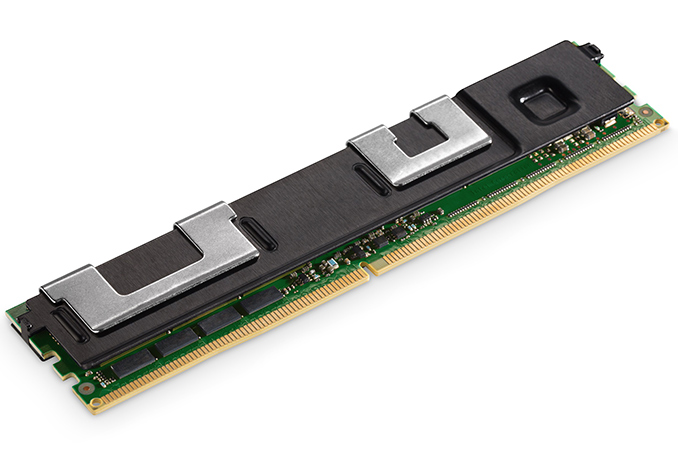
\includegraphics[width=.9\linewidth]{./IMGs/optane-module.jpg}
\end{center}

\emph{512 GB of \alert{Intel Optane DCPMM}}\\
\end{block}
\end{column}
\end{columns}
\end{frame}



\begin{frame}[label={sec:org2b7c85e}]{Intel Optane DCPMM performances}
\begin{block}{\SI{4}{\kilo\byte} direct random writes :}
\addtocounter{footnote}{-1}\\
\fontsize{10pt}{12pt}\selectfont\\
\begin{center}
\begin{tabular}{l|c|c|c|c}
 & {\color{red}DDR4 DRAM}\footnotemark & {\color{orange}Intel Optane}\footnotemark & {\color{olive}SSD} & {\color{brown}HDD}\\
\hline
Avg. Bandwidth & \SI{2.2}{\giga\byte\per\second} & \SI{790}{\mega\byte\per\second} & \SI{90}{\mega\byte\per\second} & \SI{1.5}{\mega\byte\per\second}\\
Agv. Latency & \SI{1.4}{\micro\second} & \SI{5}{\micro\second} & \SI{45}{\micro\second} & \SI{4000}{\micro\second}\\
Typical capacity & \SI{32}{\giga\byte} & 128 - \SI{512}{\giga\byte} & Some TB & 4 - 12 TB\\
Price/GB & 12 - 15 \$/GB & 4.5 - 13 \$/GB & 0.2 \$/GB & 0.1 \$/GB\\
\end{tabular}
\end{center}\footnotetext[1]{\label{orgf801544}With tmpfs\\}\footnotetext[2]{\label{orga60b0c8}ext4 (DAX)\\}
\end{block}
\end{frame}

\begin{frame}[label={sec:org1f886c0},fragile]{How to use NVMM?}
 \begin{enumerate}
\item Use \alert{PMDK} : Persistent Memory Development Kit\pause\\

\item Use a \alert{DAX} (Direct Access) file system\pause\\

\item Mmap \texttt{/dev/dax1.0} ? \pause\\

\item Something else?\\
\end{enumerate}
\end{frame}


\section{NVCache}
\label{sec:orgae53a31}

\begin{frame}[label={sec:org835d21b}]{The idea of NVCache}
\begin{columns}
\begin{column}{0.5\columnwidth}
\begin{block}{We want :}
\begin{itemize}
\item Crash resilience\pause\\

\item Performance\pause\\

\item Legacy softwares support\pause\\

\item Legacy file systems support\pause\\
\end{itemize}
\end{block}
\end{column}

\begin{column}{0.5\columnwidth}
\begin{block}{\(\Rightarrow\) Persistent Write cache}
\end{block}
\end{column}
\end{columns}
\end{frame}


\begin{frame}[label={sec:org72ae849}]{Implementation}
\begin{columns}
\begin{column}{0.6\columnwidth}
\begin{block}{Execution}
\begin{itemize}
\item A fork of the musl libc\\
\item Modifications of {\color{olive}\emph{read()}}, {\color{red}\emph{write()}}, {\color{orange}\emph{fsync()}}, etc\ldots{}\\
\item Replaces the system libc in Alpine Docker containers\\
\end{itemize}
\end{block}
\end{column}

\begin{column}{0.4\columnwidth}
\begin{block}{}
\begin{center}

\includegraphics[width=.9\linewidth]{./IMGs/musl-logo.png}
\end{center}

\begin{center}

\includegraphics[width=.9\linewidth]{./IMGs/alpine-logo.png}
\end{center}

\begin{center}

\includegraphics[width=.9\linewidth]{./IMGs/docker-logo.png}
\end{center}
\end{block}
\end{column}
\end{columns}
\end{frame}


\begin{frame}[label={sec:orgd9686df}]{Architecture}
\begin{block}{}
\begin{center}
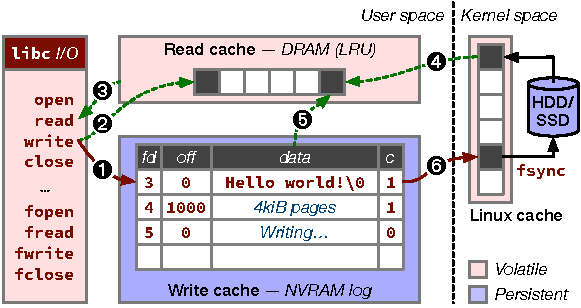
\includegraphics[width=.9\linewidth]{./IMGs/nvcache-model.pdf}
\end{center}
\end{block}
\end{frame}


\begin{frame}[label={sec:orgdce853e},fragile]{Code example}
 \begin{block}{Without NVCache:}
\fontsize{8pt}{10pt}\\
\begin{minted}[]{c}

#include<stdlib.h>
#include<unistd.h>
#include<fcntl.h>

int main(){

  char *strs[7] = {"a", "b", "c", "d", "e", "f", "g"};
  int fd = open("testfile", O_CREAT|O_RDWR);

  for(int i=0; i<7; i++){
    write(fd, strs[i], 1);
  }
  fsync(fd);
  // =========> Persistence guarantee
  close(fd);
}

\end{minted}
\end{block}
\end{frame}

\begin{frame}[label={sec:org5a9323f},fragile]{Code example}
 \begin{block}{Without NVCache:}
\fontsize{8pt}{10pt}\\
\begin{minted}[]{c}

#include<stdlib.h>
#include<unistd.h>
#include<fcntl.h>

int main(){

  char *strs[7] = {"a", "b", "c", "d", "e", "f", "g"};
  int fd = open("testfile", O_CREAT|O_RDWR);

  for(int i=0; i<7; i++){
    write(fd, strs[i], 1); // Crash?
  }
  fsync(fd);
  // =========> Persistence guarantee
  close(fd);
}

\end{minted}
\end{block}
\end{frame}

\begin{frame}[label={sec:org55bf938},fragile]{Code example}
 \begin{block}{With NVCache:}
\fontsize{8pt}{10pt}\\
\begin{minted}[]{c}

#include<stdlib.h>
#include<unistd.h>
#include<fcntl.h>

int main(){

  char *strs[7] = {"a", "b", "c", "d", "e", "f", "g"};
  int fd = open("testfile", O_CREAT|O_RDWR);

  for(int i=0; i<7; i++){
    write(fd, strs[i], 1);
  // ========================> Persistence guarantee
  }
  fsync(fd); // Does nothing
  close(fd); // Flushes NVM => Disk
}

\end{minted}
\end{block}
\end{frame}

\begin{frame}[label={sec:org90b9e4a},fragile]{Code example}
 \begin{block}{With NVCache:}
\fontsize{8pt}{10pt}\\
\begin{minted}[]{c}

#include<stdlib.h>
#include<unistd.h>
#include<fcntl.h>

int main(){

  char *strs[7] = {"a", "b", "c", "d", "e", "f", "g"};
  int fd = open("testfile", O_CREAT|O_RDWR);

  for(int i=0; i<7; i++){
    write(fd, strs[i], 1); // Crash?
  // ========================> Persistence guarantee
  }
  fsync(fd); // Does nothing
  close(fd); // Flushes NVM => Disk
}

\end{minted}
\end{block}
\end{frame}


\begin{frame}[label={sec:orgfe7392d}]{Benchmarks}
\begin{block}{\SI{4}{\kibi\byte} random writes}
\begin{center}
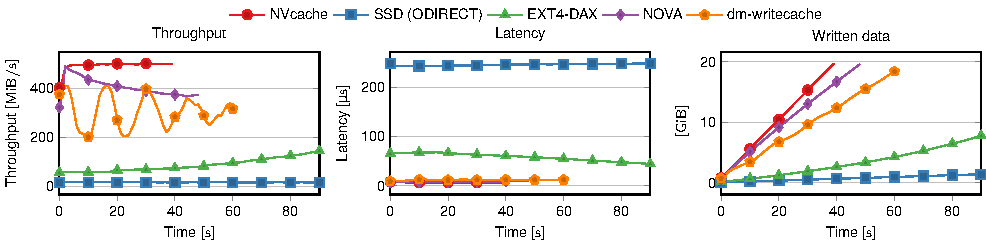
\includegraphics[width=.9\linewidth]{./IMGs/paper-figure1.pdf}
\end{center} \pause\\

\begin{center}
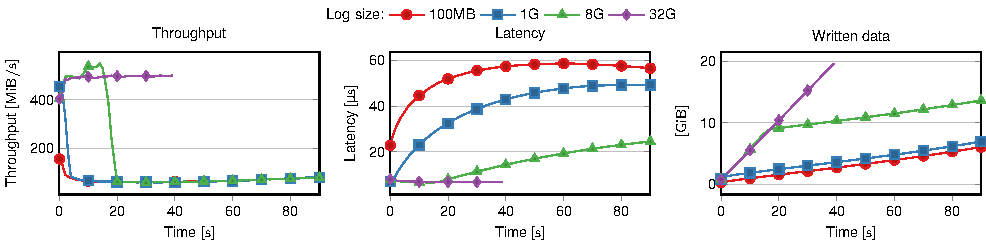
\includegraphics[width=.9\linewidth]{./IMGs/paper-figure2.pdf}
\end{center}
\end{block}
\end{frame}


\section{The End}
\label{sec:org6e5c8fa}

\begin{frame}[label={sec:orgb9f9629}]{NVCache: Conclusion}
\begin{columns}
\begin{column}{0.6\columnwidth}
\begin{block}{We managed to:}
\begin{itemize}
\item Add new guarantees\\
\item Keep good performances\\
\item Exceed the limited NVM capacity\\
\end{itemize}
\end{block}
\end{column}

\begin{column}{0.4\columnwidth}
\begin{block}{\(\Rightarrow\) Less than 3000 lines of code}
\end{block}
\end{column}
\end{columns}
\end{frame}

\begin{frame}[label={sec:org7dab81a}]{Thank you for your attention!}
\begin{columns}
\begin{column}{0.4\columnwidth}
\begin{block}{}
Questions?\\
\end{block}
\end{column}


\begin{column}{0.6\columnwidth}
\begin{block}{}
\begin{center}
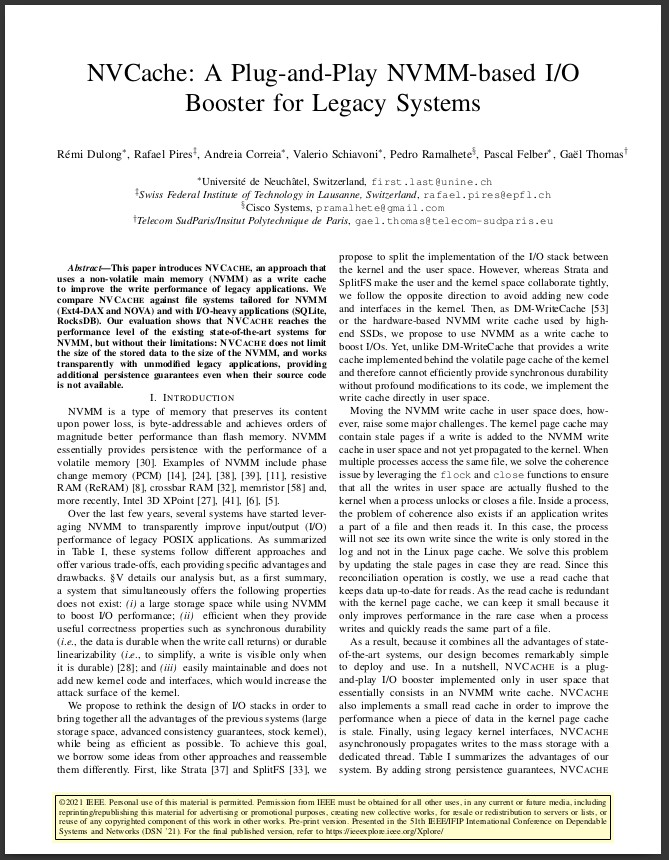
\includegraphics[width=.9\linewidth]{./IMGs/paper.jpg}
\end{center}
\end{block}
\end{column}
\end{columns}
\end{frame}



\begin{frame}[label={sec:orgadbd897}]{Authors}
\fontsize{5pt}{7pt}\\

\begin{block}{}
\begin{columns}
\begin{column}{0.2\columnwidth}
\begin{block}{Rémi Dulong}
University of Neuchâtel\\
\begin{center}

\includegraphics[width=.9\linewidth]{./IMGs/remi.jpg}
\end{center}
\end{block}
\end{column}

\begin{column}{0.2\columnwidth}
\begin{block}{Rafael Pires}
University of Neuchâtel\\
\begin{center}
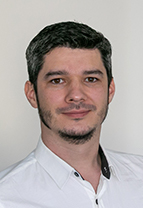
\includegraphics[width=.9\linewidth]{./IMGs/rafael.jpg}
\end{center}
\end{block}
\end{column}

\begin{column}{0.2\columnwidth}
\begin{block}{Andreia Correia}
University of Neuchâtel\\
\begin{center}
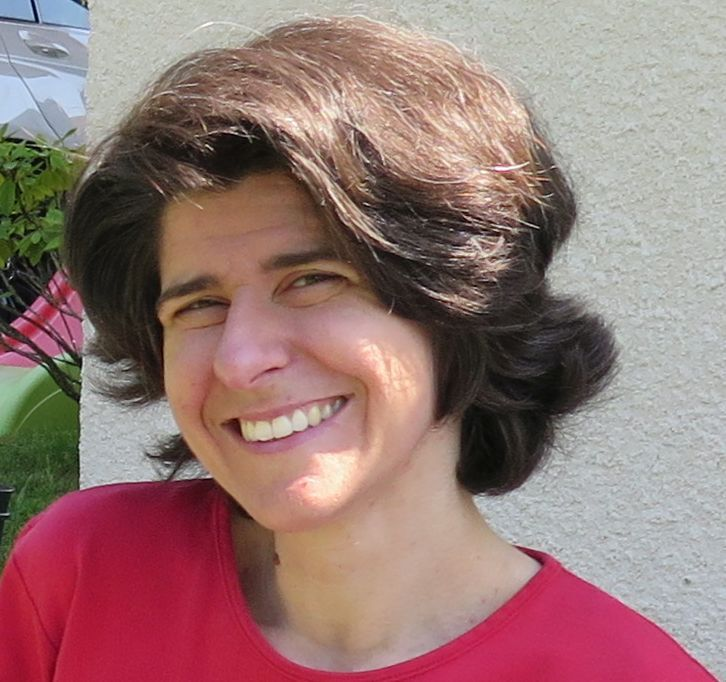
\includegraphics[width=.9\linewidth]{./IMGs/andreia.jpg}
\end{center}
\end{block}
\end{column}
\begin{column}{0.2\columnwidth}
\begin{block}{Pedro Ramalhete}
Cicso systems\\
\begin{center}
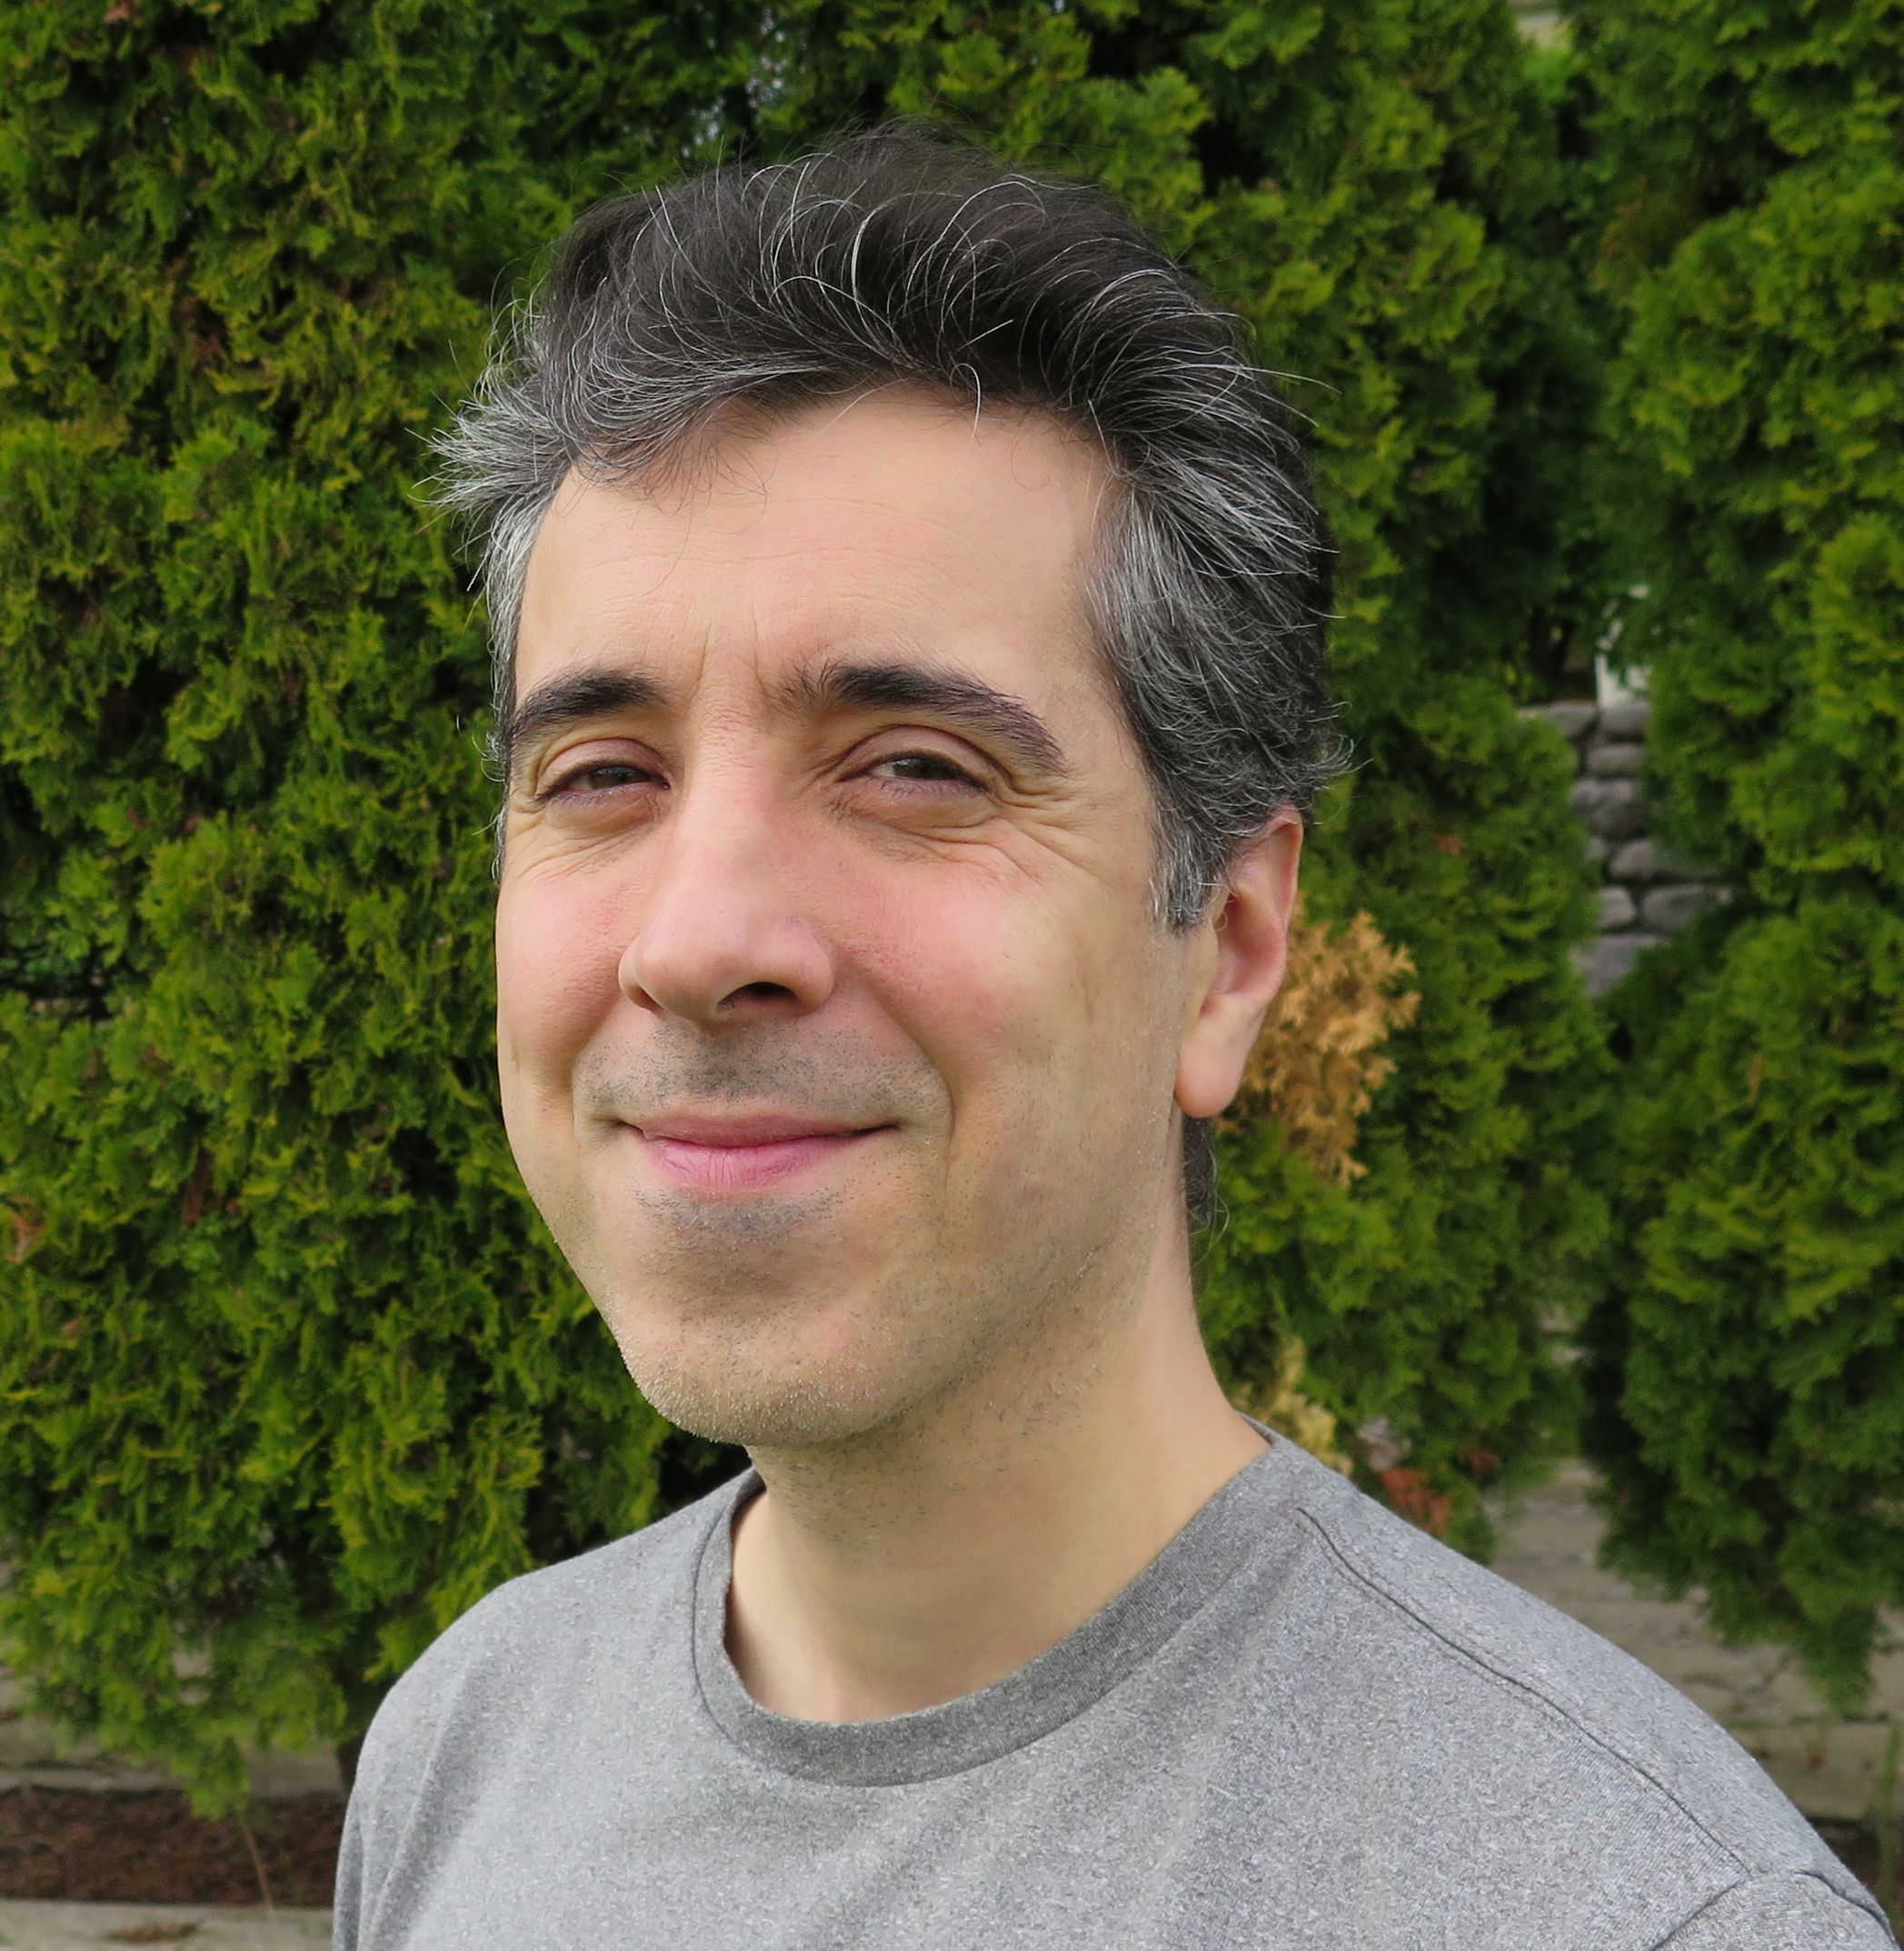
\includegraphics[width=.9\linewidth]{./IMGs/pedro.jpg}
\end{center}
\end{block}
\end{column}
\end{columns}
\end{block}

\begin{block}{}
\begin{columns}
\begin{column}{0.2\columnwidth}
\begin{block}{Pascal Felber}
University of Neuchâtel\\
\begin{center}
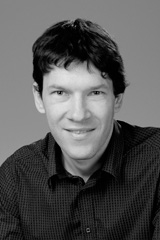
\includegraphics[width=.9\linewidth]{./IMGs/pascal.jpg}
\end{center}
\end{block}
\end{column}

\begin{column}{0.2\columnwidth}
\begin{block}{Gaël Thomas}
Télécom SudParis\\
\begin{center}
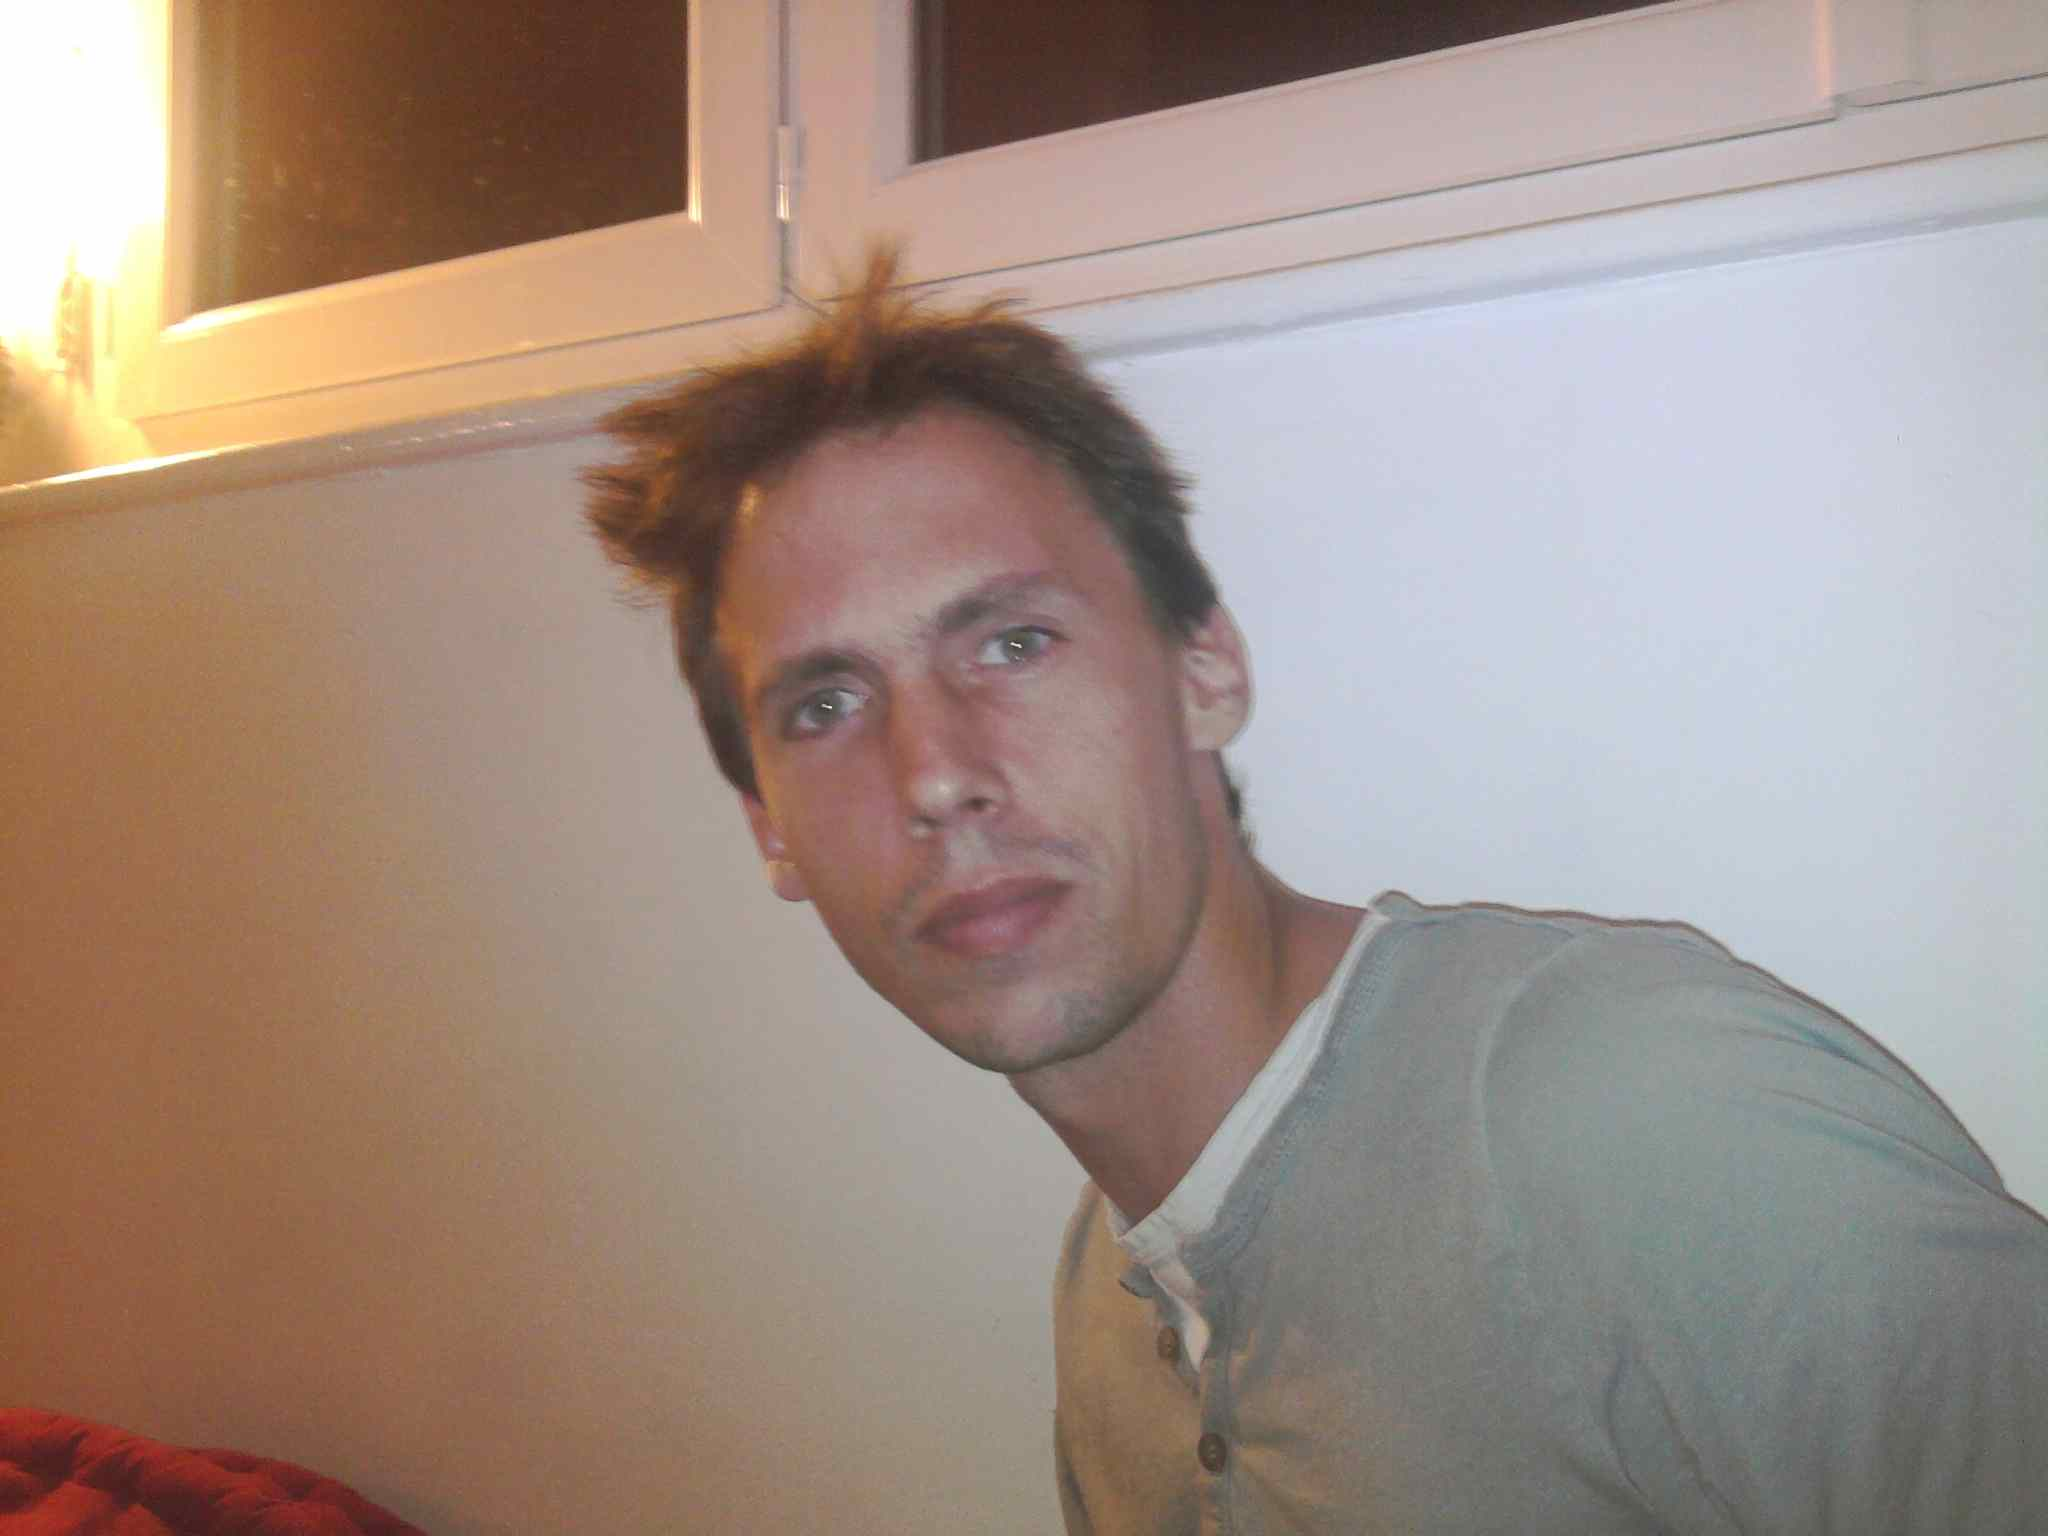
\includegraphics[width=.9\linewidth]{./IMGs/gael.jpg}
\end{center}
\end{block}
\end{column}

\begin{column}{0.2\columnwidth}
\begin{block}{Valerio Schiavoni}
University of Neuchâtel\\
\begin{center}
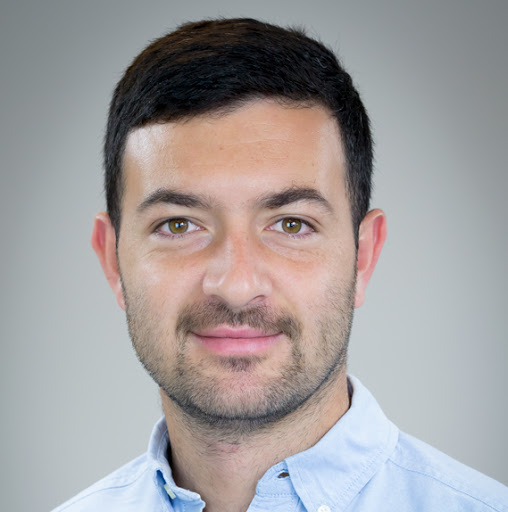
\includegraphics[width=.9\linewidth]{./IMGs/valerio.jpg}
\end{center}
\end{block}
\end{column}
\end{columns}
\end{block}
\end{frame}

\begin{frame}[label={sec:orgd119ba7}]{End}
\uline{\emph{Contact :}} Rémi Dulong, remi.dulong@unine.ch\\
\end{frame}
\end{document}
